% Praktischer Teil
\section{Results}
\label{sec:results}

\subsection{Included Weather Stations}

From the 3D-Paws project of NCAR, measurements from three different weather stations in recent years were obtained. The stations are located in Marshall, Colorado; Vienna, Austria; and Barbados, Caribbean. The measurements span up to late 2023, with the quantity of available temperature data varying significantly between stations. The station in Marshall is one of the oldest in the 3D-Paws project and has the most available measurements among the three stations. The weather station in Vienna also has data dating back to 2017, but it has been almost completely offline since mid-2019. The weather station in Barbados began recording in mid-2020

% 3 images side by side with available weather stations
\begin{figure}
    \centering
    \begin{subfigure}{0.672\textwidth}
        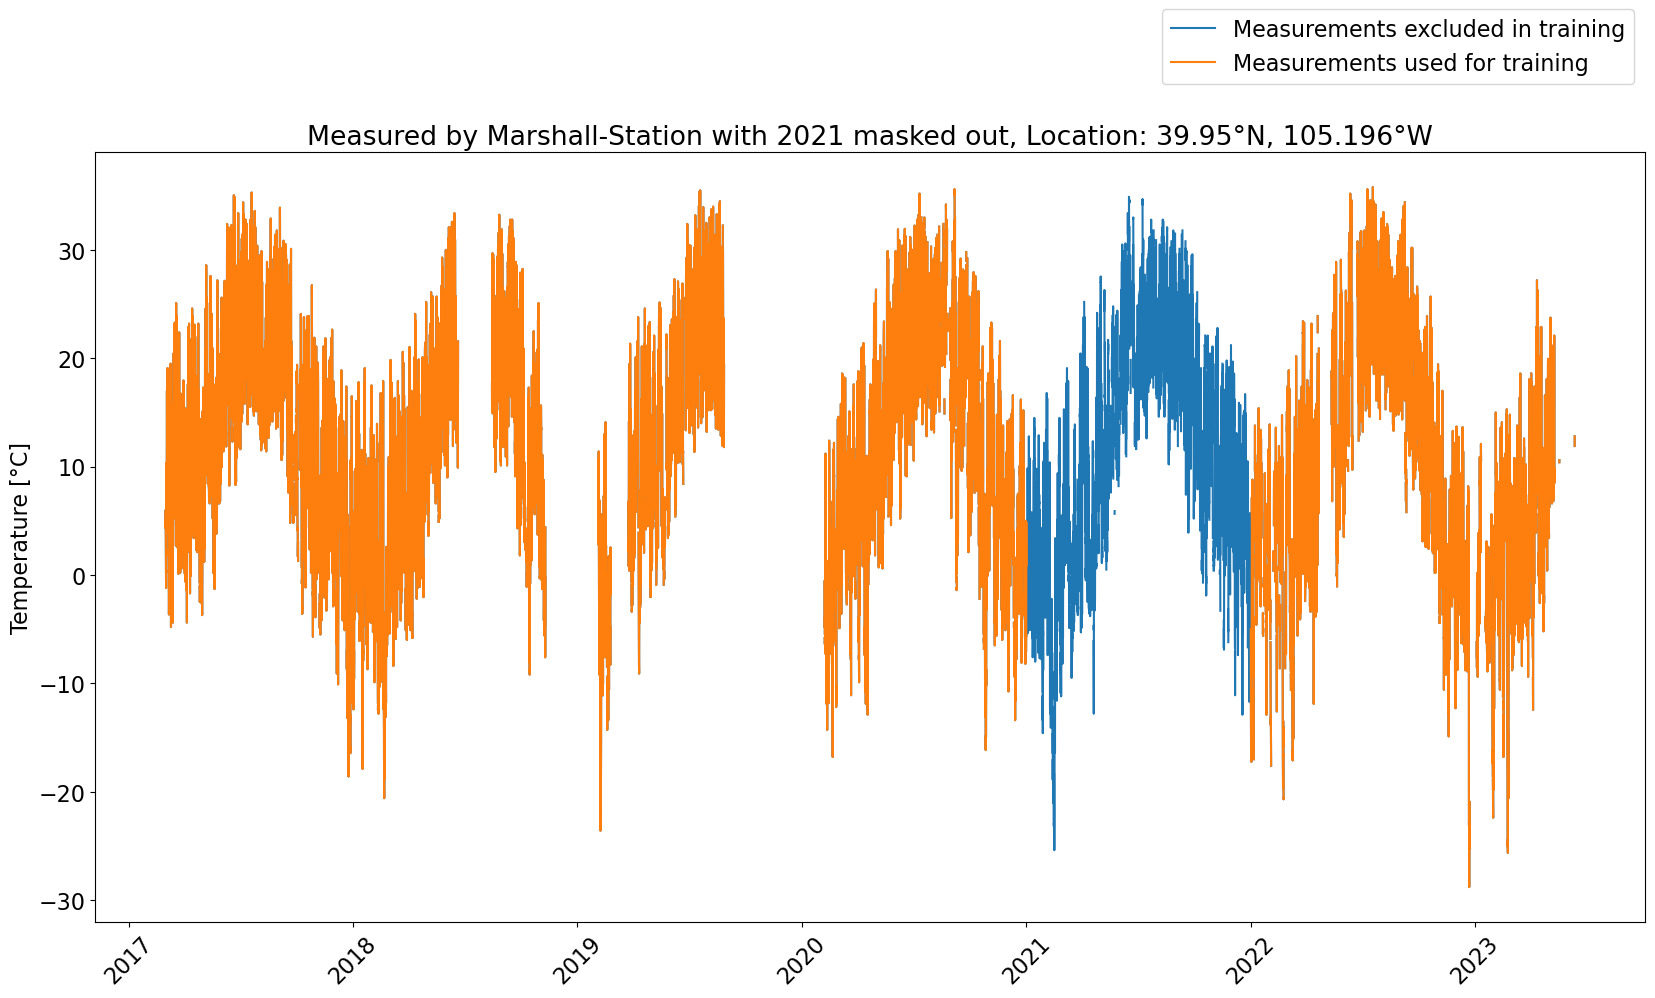
\includegraphics[width=\textwidth]{resources/images/charts/marshall_available_measurements.png}
        \caption{Station in Marshall, Colorado, USA}
        \label{fig:available_measurements_marshall}
    \end{subfigure}
    \begin{subfigure}{0.672\textwidth}
        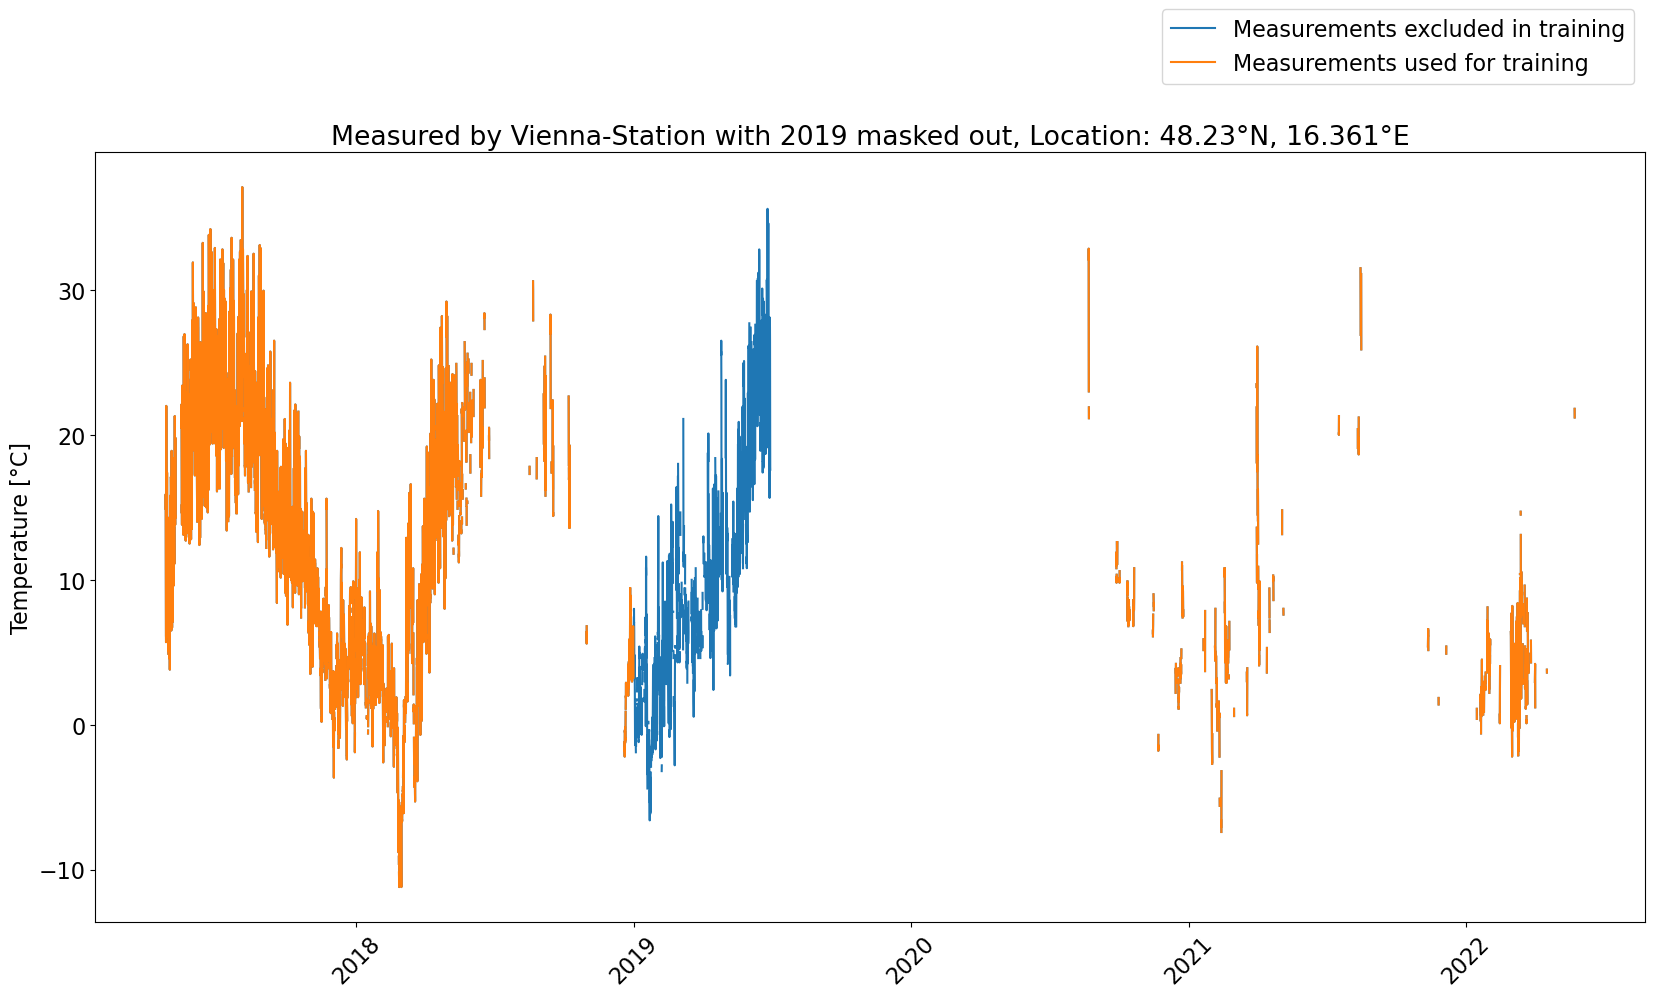
\includegraphics[width=\textwidth]{resources/images/charts/vienna_available_measurements.png}
        \caption{Station in Vienna, Austria}
        \label{fig:available_measurements_vienna}
    \end{subfigure}
    \begin{subfigure}{0.672\textwidth}
        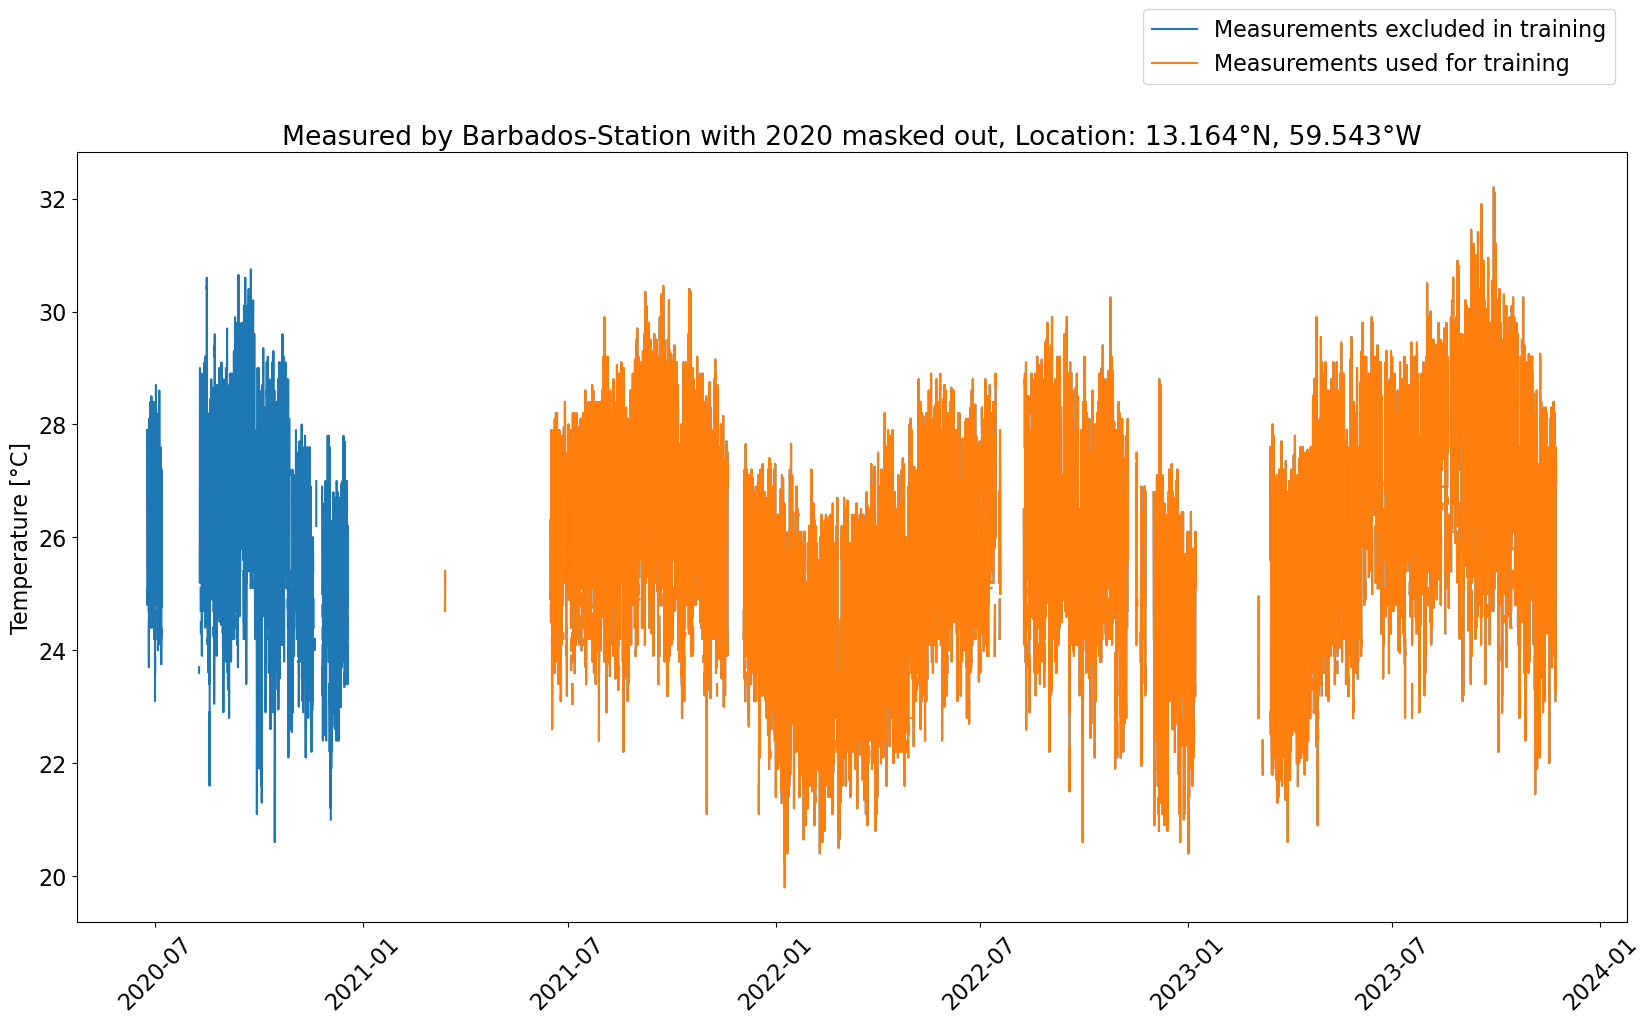
\includegraphics[width=\textwidth]{resources/images/charts/barbados_available_measurements.png}
        \caption{Station in Barbados, Caribbean}
        \label{fig:available_measurements_barbados}
    \end{subfigure}
    \caption{Available data from 3D printed Weather stations}
    \label{fig:weather_stations}
\end{figure}

\begin{wrapfigure}[15]{r}{0.36\textwidth}
    \centering
    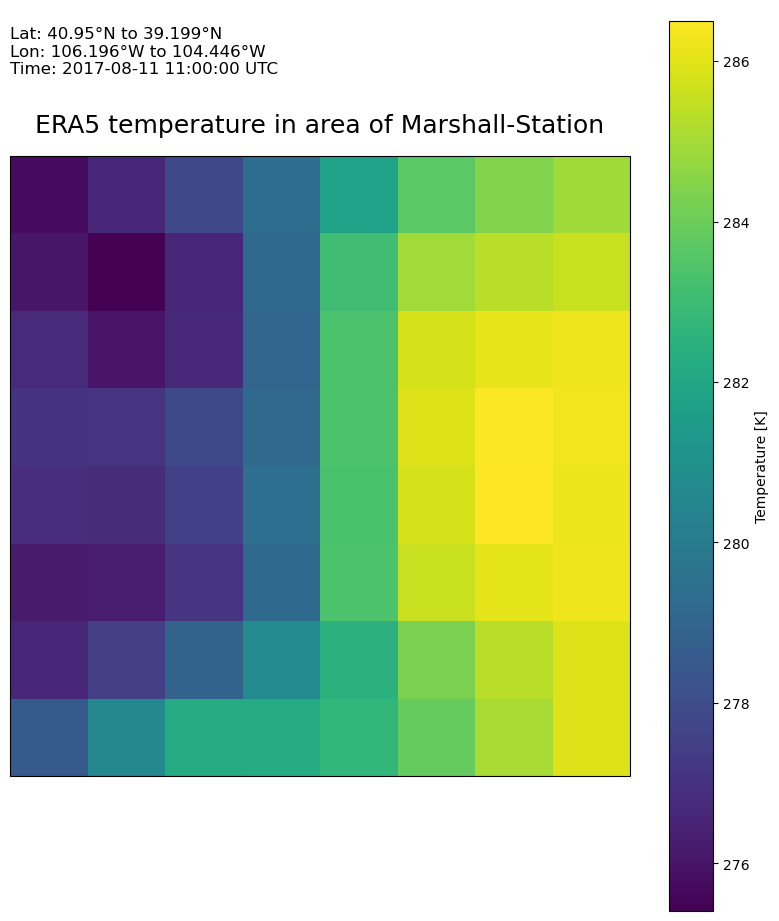
\includegraphics[width=0.35\textwidth]{resources/images/Marshall_era5.png}
    \caption{ERA5 Area of the station in Marshall, Colorado}
    \label{fig:era5_marshall}
\end{wrapfigure}


The station in Marshall is located between Boulder and Denver next to Marshall Lake, on an Elevation of 1743m, less than 10km east of the South Boulder Peak, which is already more than 2600m high \cite{southboulderpeak}. That the station is located just about 30 kilometers east of the Colorado Front Range where the Rocky Mountains range in their altitude between 3250m - 4000m \cite{Williams1996} is visible in the ERA5 data \autoref{fig:era5_marshall}.

Vienna is situated to the west within the Vienna Basin, at a relatively low altitude just beyond the Alpine region. The Alps, which rise moderately western of Vienna, reach heights of up to 2000 meters above sea level in a distance of approximately 100km, meaning the ERA5 resolution is high enough to differentiate the atmospheric conditions and topographical features within this region better.

The station in Barbados is located in the parish of St George at an altitude of 274m, the island itself is relatively flat with the highest point being Mount Hillaby at 340m. The island is 34km long and up to 23km wide, which is approximately the size of an ERA5 grid cell, but as can be observed in \autoref{fig:barbados} all surrounding grid cells are ocean heavy, while the stations location on Barbados is close the the point where the landmass is the widest. The ERA5 data is therefore not able to capture the diurnal cycle of the station as it is located on land, while the surrounding grid cells are mostly ocean.

\subsection{Data availability}
In \autoref{fig:weather_stations} the measurements of the three stations are displayed, after data cleansing and converting them on an hourly basis. The measurements were provided by the NCAR with most invalid values already marked as such but especially in Barbados the sensors had more noise and occasional invalid measurements such that they needed extra cleansing. To do so, values at temperatures near zero and below were excluded. The conversion from minute to hourly data was done by taking the average of all minute values in that specific hour, but only if there were more than 20 values available and only if the values weren't all the same. It has been observed that the sensors sometimes get stuck and then deliver the same value for a longer period. The dataset for the Marshall station spans from 2017 to 2023, comprising 41,883 data points. These measurements reveal three significant data gaps along with several smaller ones. The larger intervals without data include the midsummer period of 2018, late 2019 to early 2020, and the most extensive gap occurring over five months from September 2019 to January 2020

For the Vienna Station, measurements are available for only 12,477 hours, which is less than a third compared to Marshall. This is primarily due to extended downtimes starting from mid-2018, resulting in few to no measurement data. Except for a brief period from late 2018 to July 2019, when continuous measurements resumed. After that, there were only sporadic data collection instances, before the station went preliminary offline in April 2022.

The Barbados Station only suffered 2 downtimes that were significantly longer than a month with the biggest being roughly the first half of 2021 and the 2nd biggest being the first quarter of 2023. In total the station has 17,315 hours of measurements, which is still less than half of the Marshall station. 

\subsection*{Splitting into Training and Validation Data}

As explained in \autoref{sec:design}, the measurements are split into a training and validation dataset. The training dataset is used to train the model, while the validation dataset will be kept aside to compare it to what the model predicts after the training to validate if and to which extent the model learned to reconstruct the missing data. If the validation data would be included in the training data, the model would be able to predict the values it has already seen, but it would be impossible to tell if the model learned to generalize the local wather patterns.
Starting with the Marshall station, the data was sufficient to extract an entire year as validation data. Excluding a consecutive year from the training data not only allows for a comprehensive analysis of a full yearly cycle but also ensures that the model relies solely on the general weather patterns it learned from the training data to predict the values of the validation data. This approach prevents the model from potentially "cheating" by accessing information from nearby training data points, which could compromise the integrity of the validation process. It is a common practice in the machine learning field to validate data as a contiguous set, as it helps to maintain the independence and integrity of the validation process. 2021 highlighted in blue in \ref{fig:available_measurements_marshall} was the most complete year in the Marshall dataset thus it was chosen as the validation data. With the mask of 2021 applied the training data for Marshall consists of 34,188 hours of measurements which is about 82\% of the total data.

For the Vienna station, the data was split into training and validation data based on the availability of the data. The training data consists of all available data up to 2019, while the validation data is the year 2019. Resulting in 9,593 hours of measurements used as training data, which is about 77\% of the total data. The limited availability of measurements didn't allow for a full year of validation data.

The Barbados station also only had 2022 and 2023 as a complete available years, so that the decision to use the available data of 2020 as a training was a result of the lack of data as well. With the mask applied, the training data consists of 14,576 hours of measurements, which is about 84\% of the total data.


% Marshall 41883, 34188 without 2021 -> gives a ratio for validation data of 0.18

% Barbados 17315, 14576 without 2020 -> gives a ratio for validation data of 0.16

% Vienna 12477, 9593 without 2019 -> gives a ratio for validation data of 0.23


\subsection{Validation of the Model}
\subsection*{Marshall Station}

\begin{figure}
    \centering
    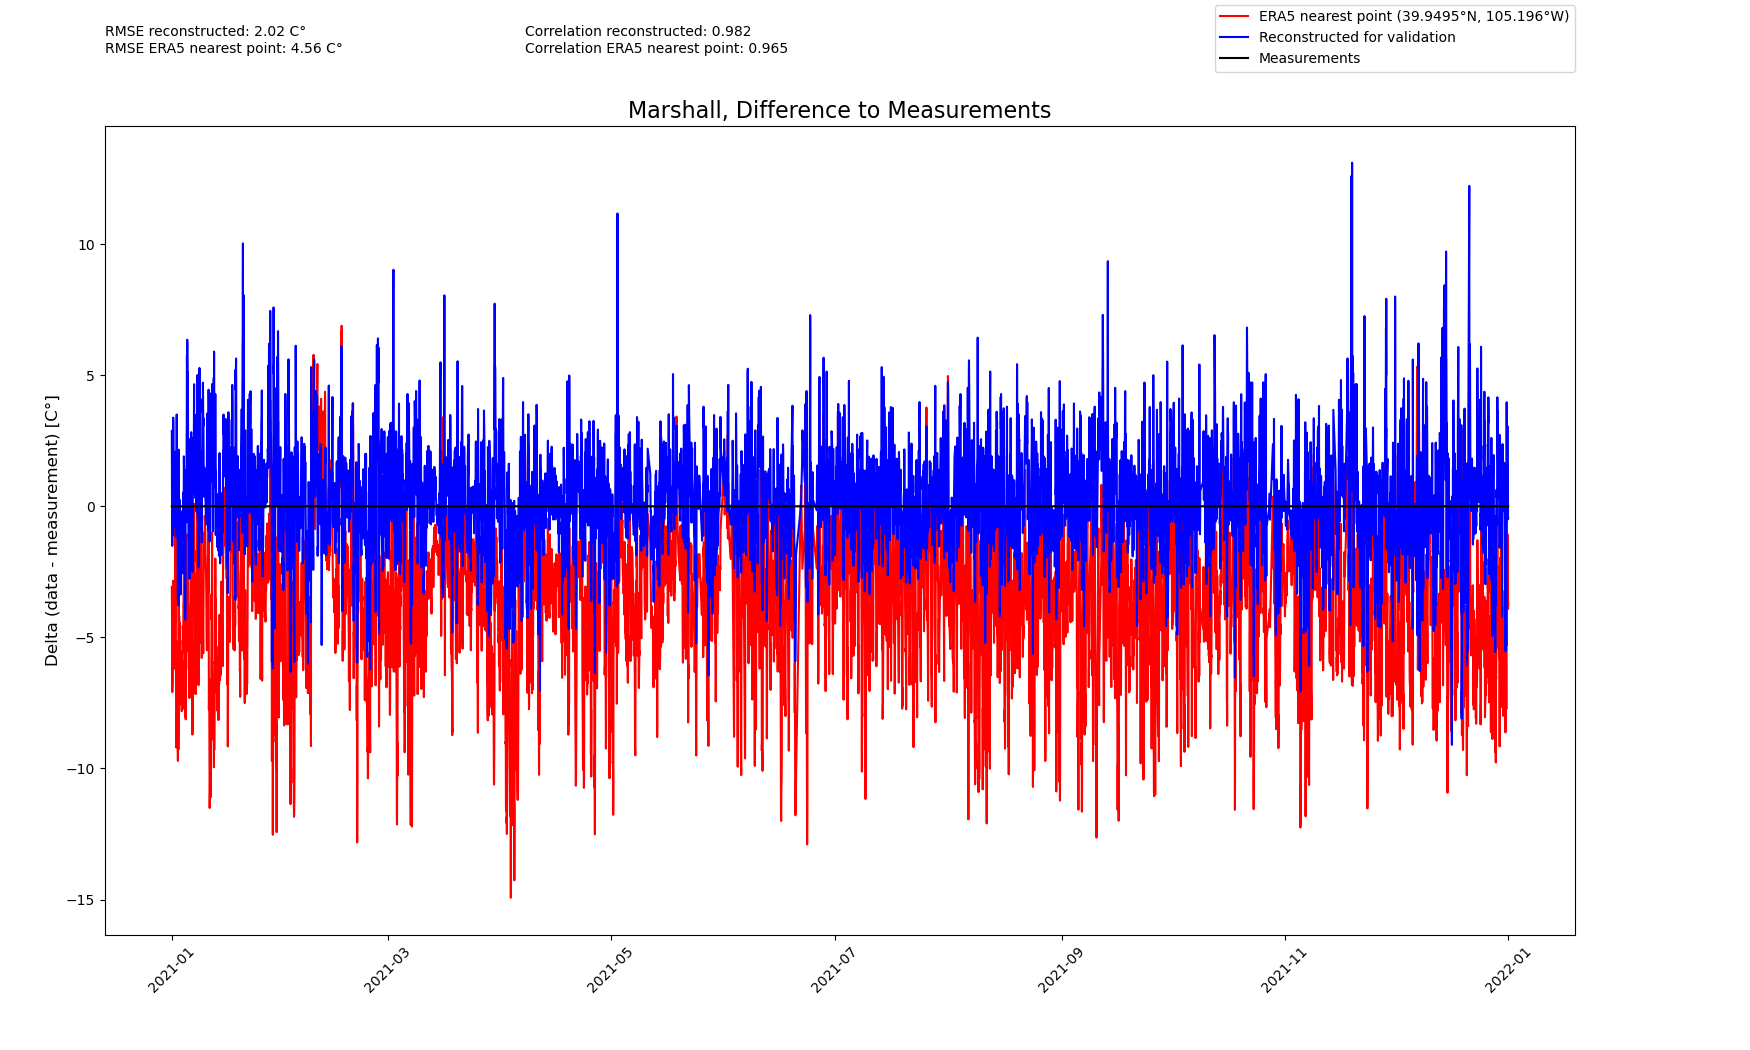
\includegraphics[width=\textwidth]{resources/images/charts/marshall_eval_grib_final/Marshall, Difference to Measurements.png}
    \caption{Difference between reconstructed and measured temperature for Marshall-Station}
\end{figure}

\begin{figure}
    \centering
    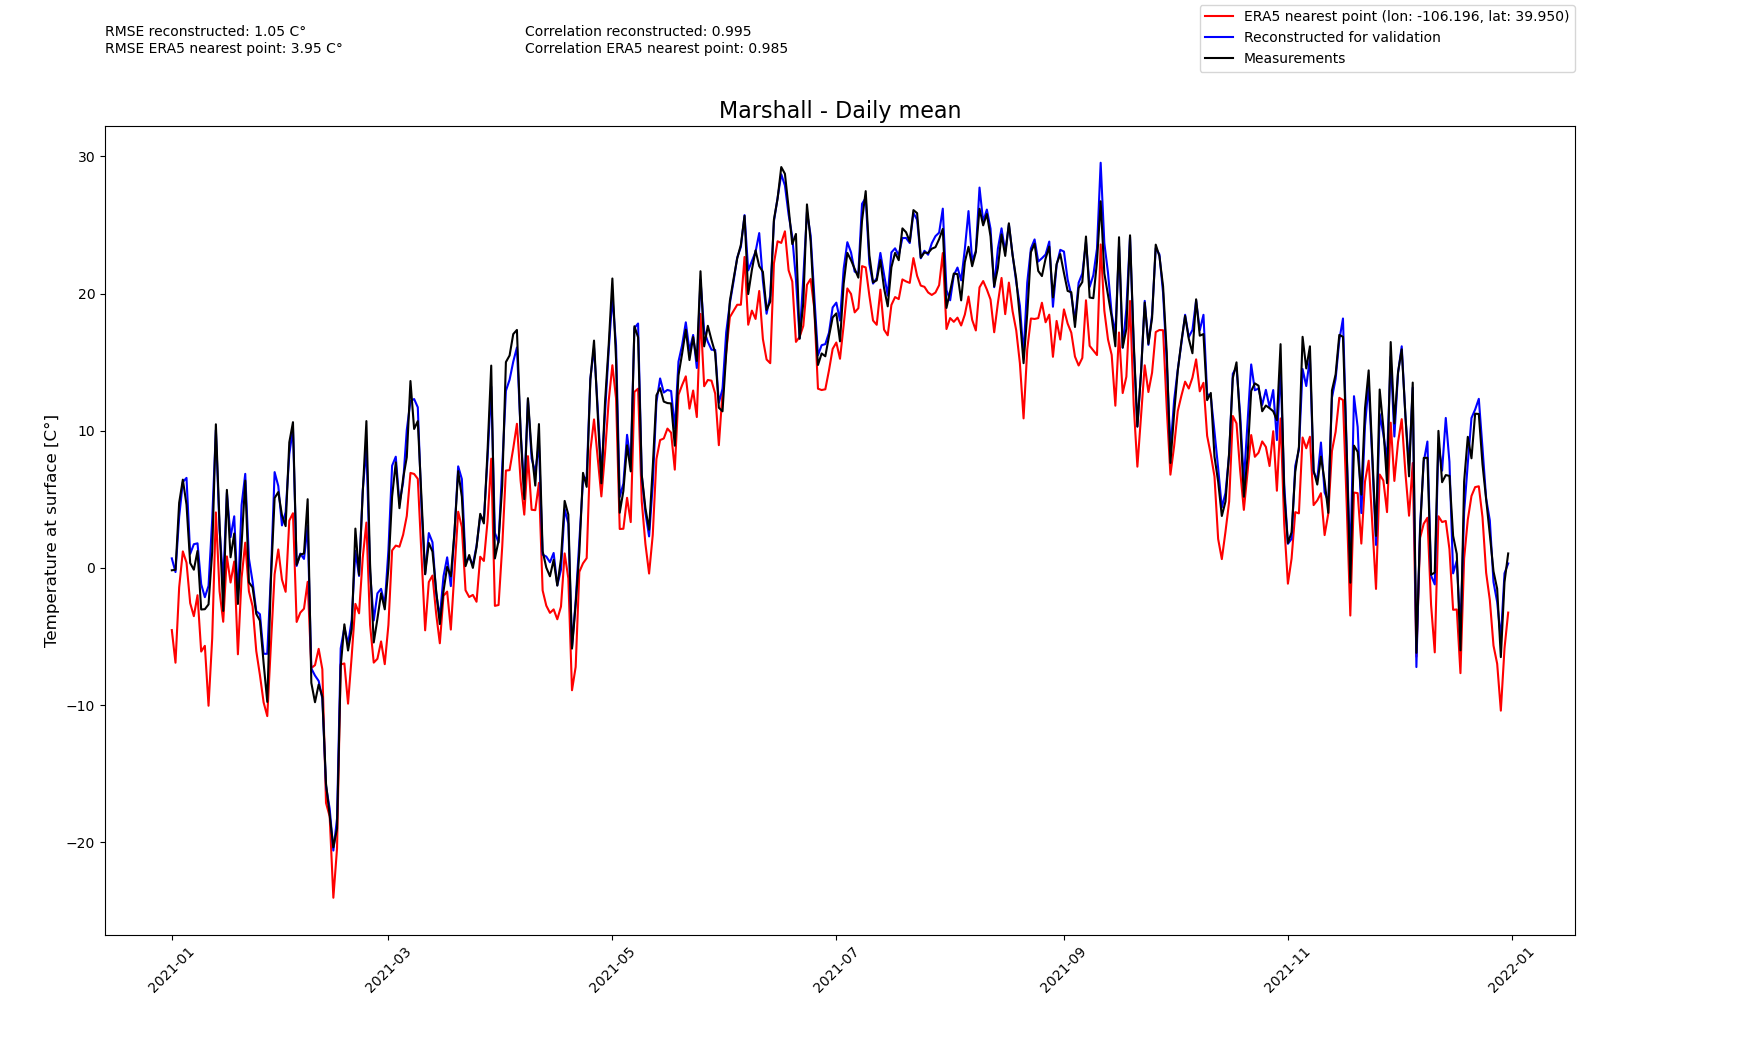
\includegraphics[width=\textwidth]{resources/images/charts/marshall_eval_grib_final/Marshall - Daily mean.png}
    \caption{Reconstructed temperature vs measured temperature for Marshall-Station (Daily mean)}
\end{figure}

\begin{figure}
    \centering
    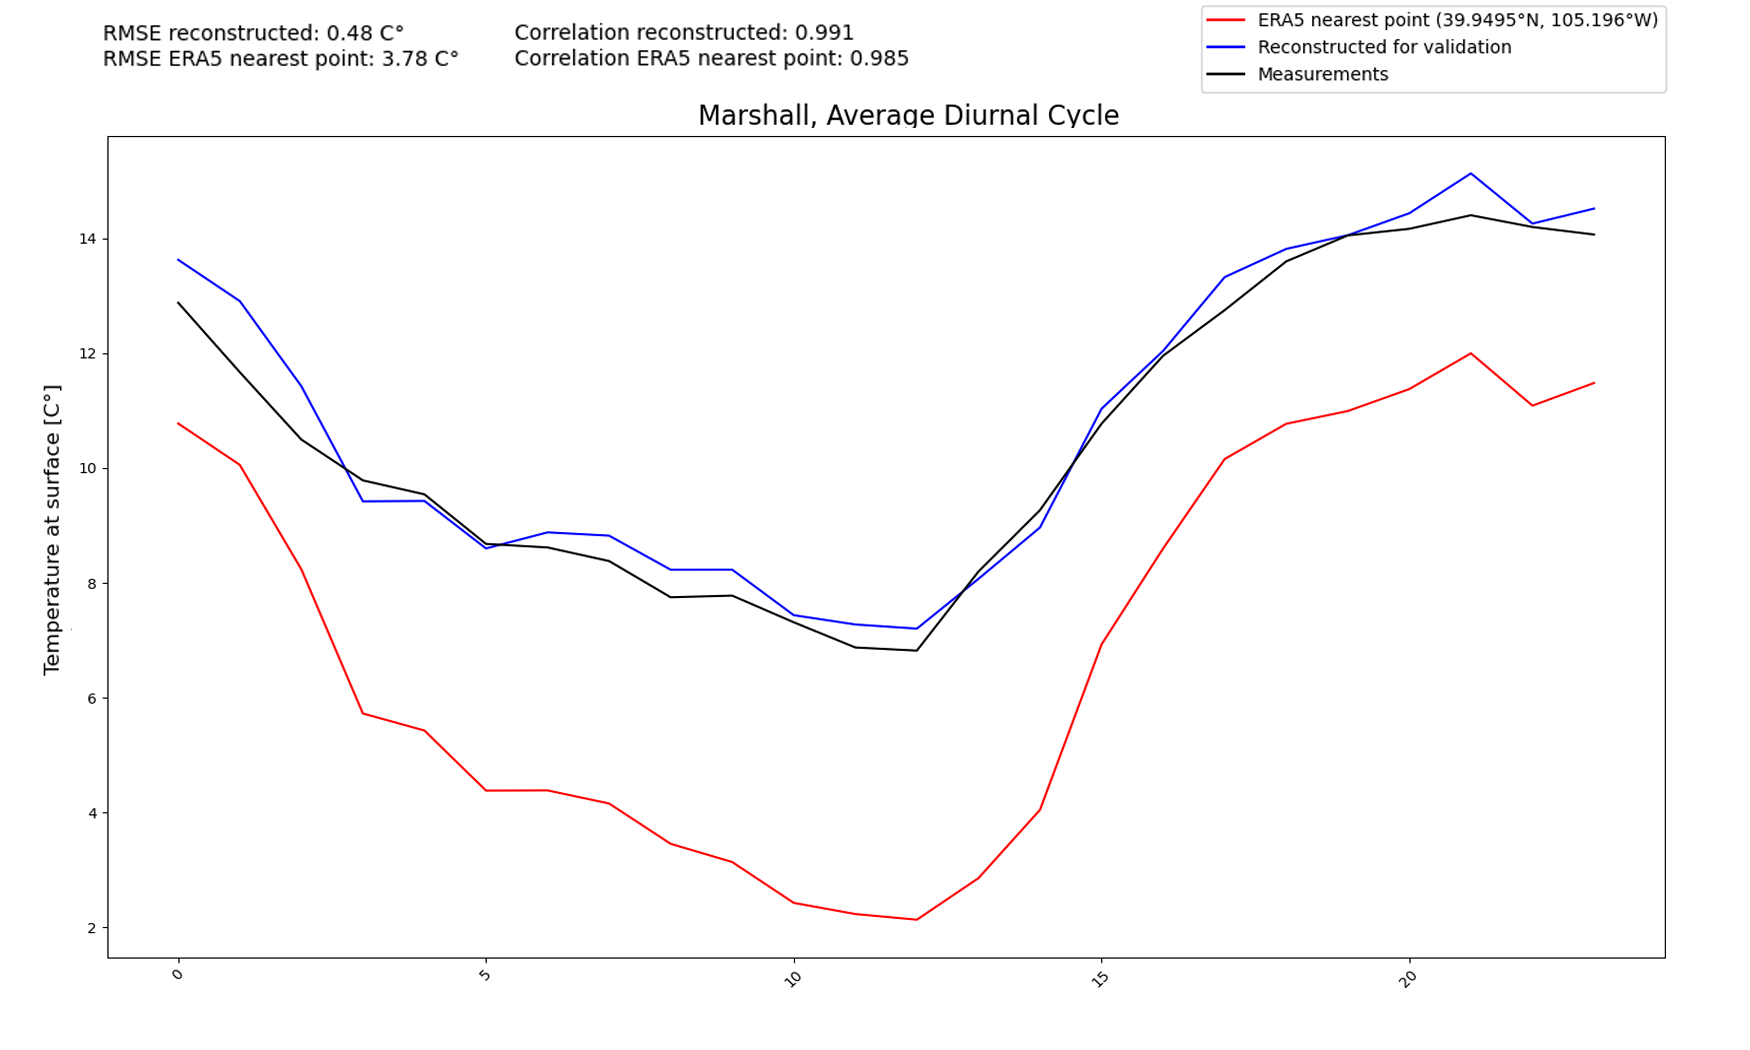
\includegraphics[width=\textwidth]{resources/images/charts/marshall_eval_grib_final/Marshall, Average Diurnal Cycle.png}
    \caption{Reconstructed temperature vs measured temperature for Marshall-Station (Average Diurnal Cycle)}
\end{figure}

\begin{figure}
    \centering
    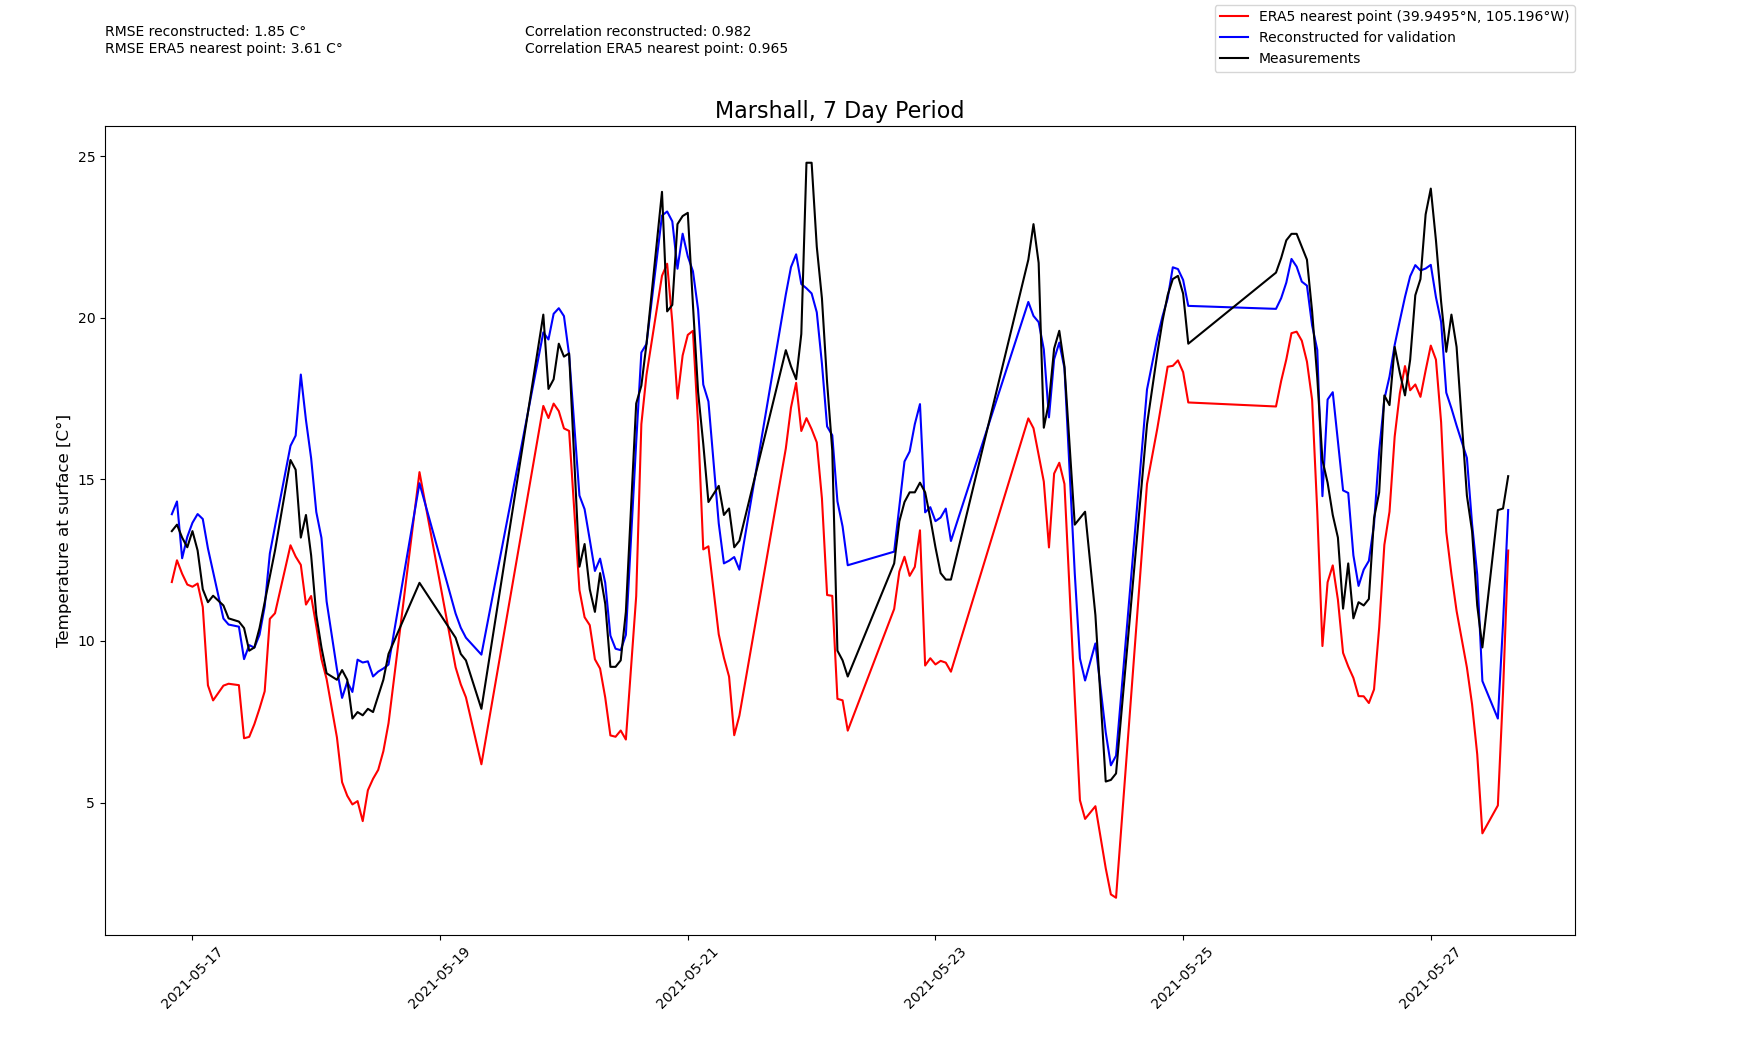
\includegraphics[width=\textwidth]{resources/images/charts/marshall_eval_grib_final/Marshall, 7 Day Period_1_2_3.png}
    \caption{Reconstructed temperature vs measured temperature for Marshall-Station (7 Day Period)}
\end{figure}

\begin{figure}
    \centering
    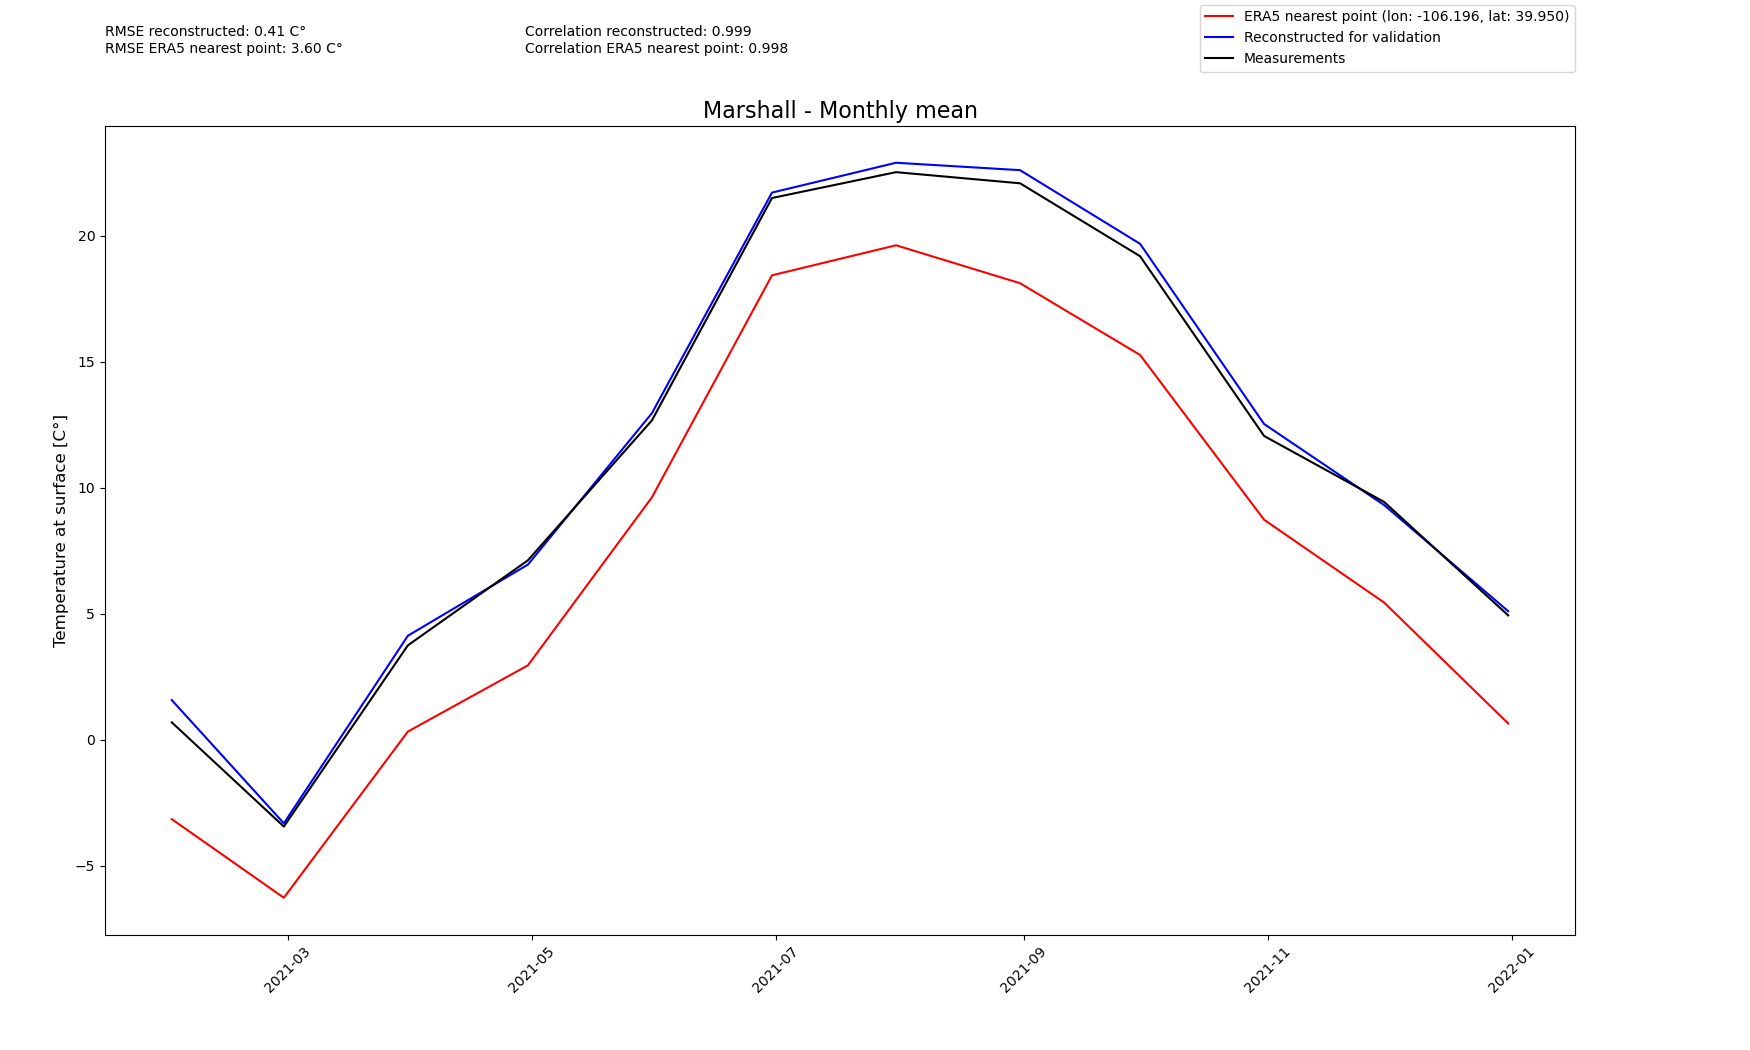
\includegraphics[width=\textwidth]{resources/images/charts/marshall_eval_grib_final/Marshall - Monthly mean.png}
    \caption{Reconstructed temperature vs measured temperature for Marshall-Station (Monthly mean)}
\end{figure}

\newpage

\subsection*{Vienna Station}

\begin{figure}
    \centering
    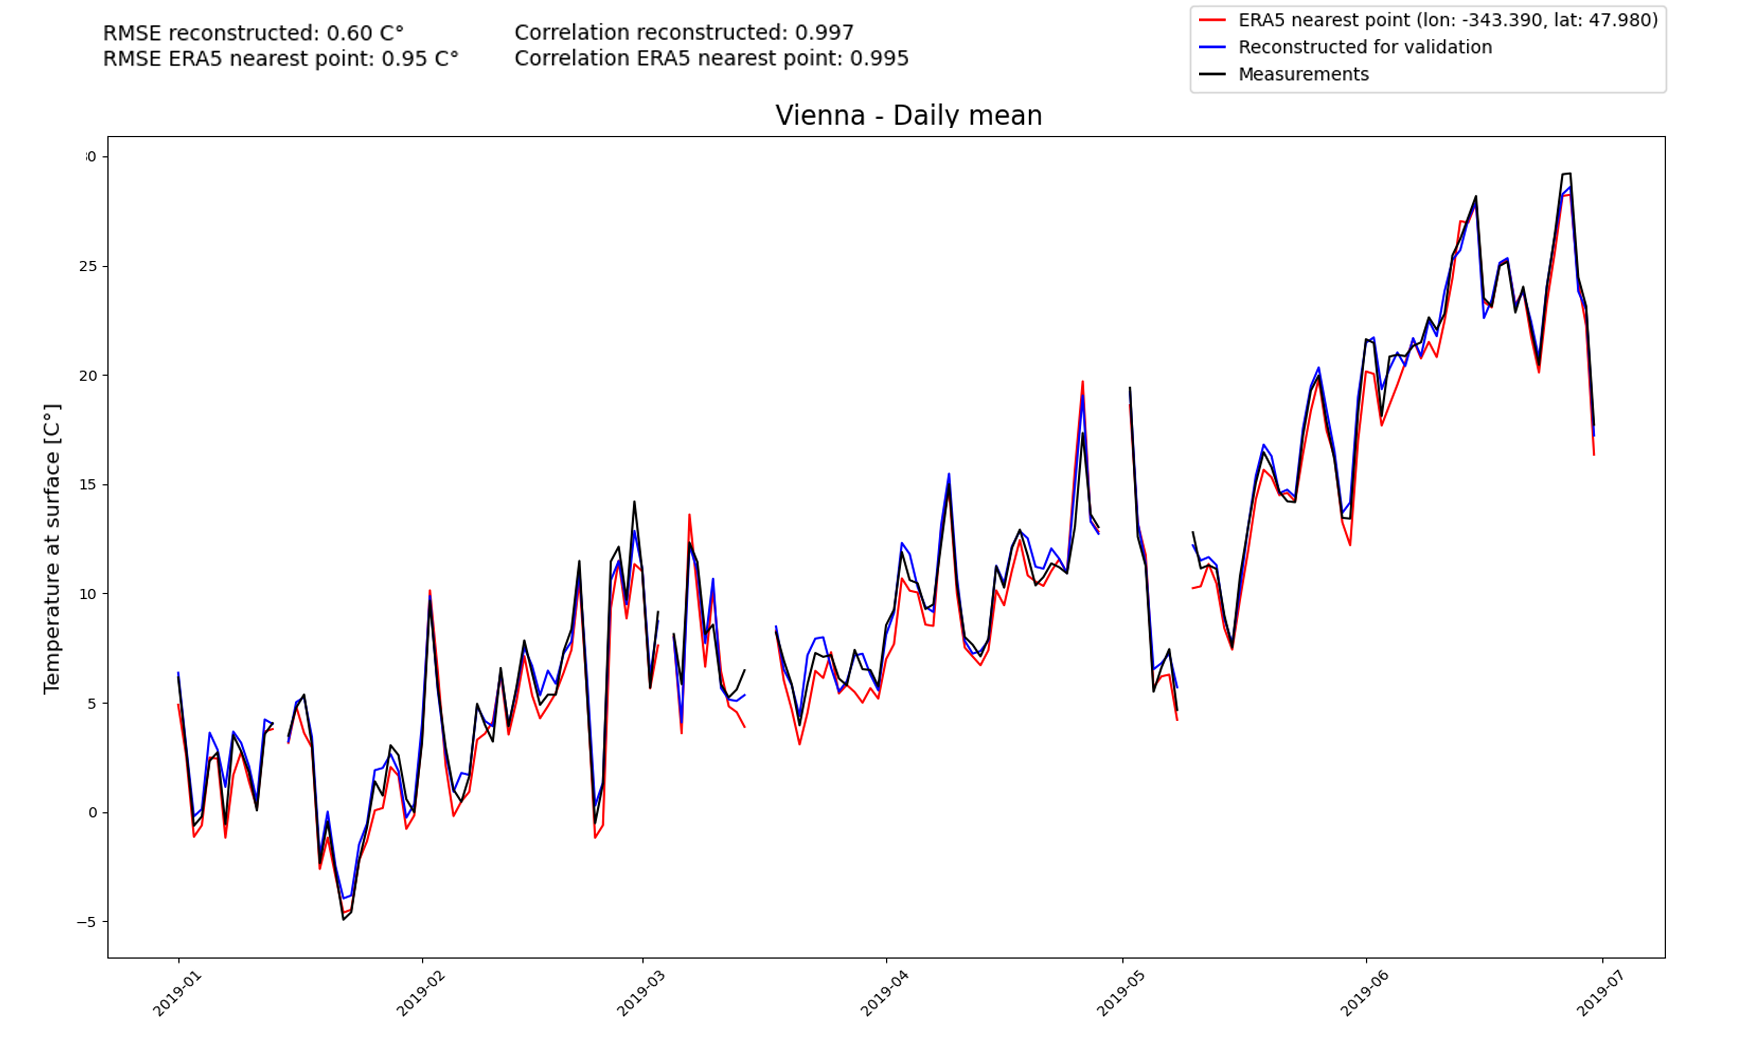
\includegraphics[width=\textwidth]{resources/images/charts/vienna_eval_grib_final/Vienna - Daily mean.png}
    \caption{Reconstructed temperature for Vienna-Station (Daily mean)}
\end{figure}

\begin{figure}
    \centering
    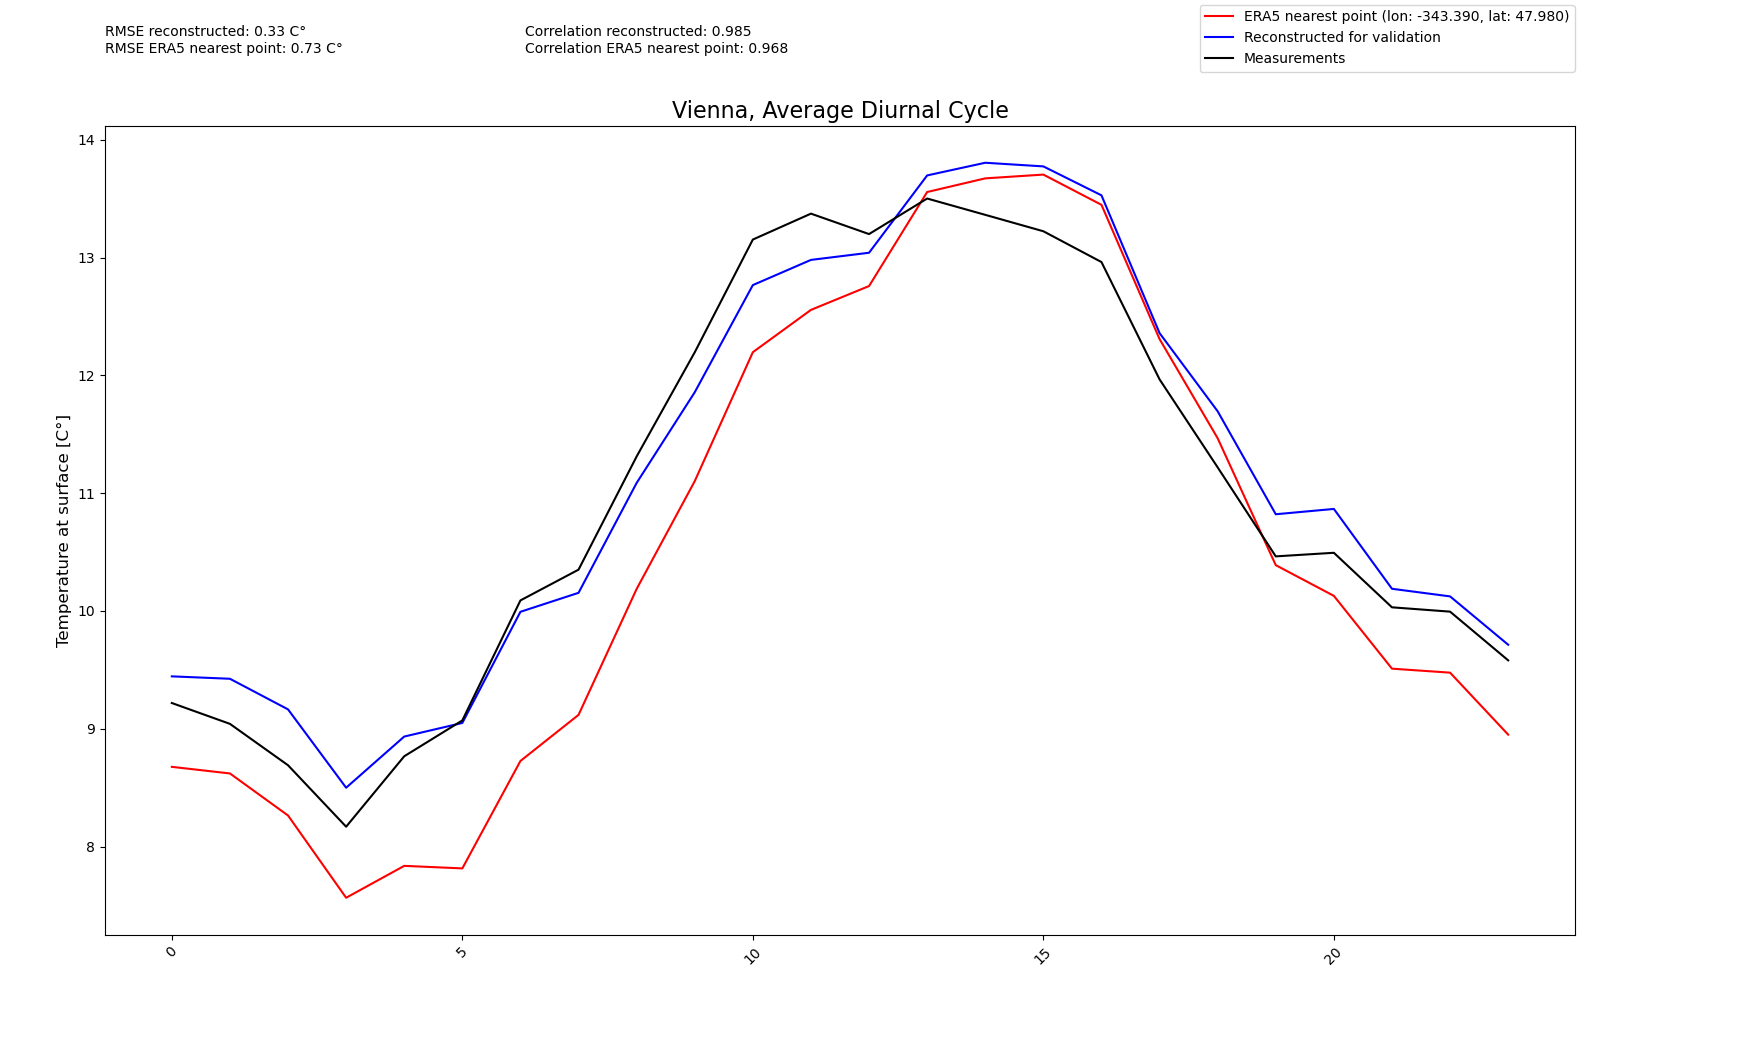
\includegraphics[width=\textwidth]{resources/images/charts/vienna_eval_grib_final/Vienna, Average Diurnal Cycle.png}
    \caption{Measured temperature for Vienna-Station (Average Diurnal Cycle)}
\end{figure}

\newpage

\subsection*{Barbados Station}

\begin{figure}
    \centering
    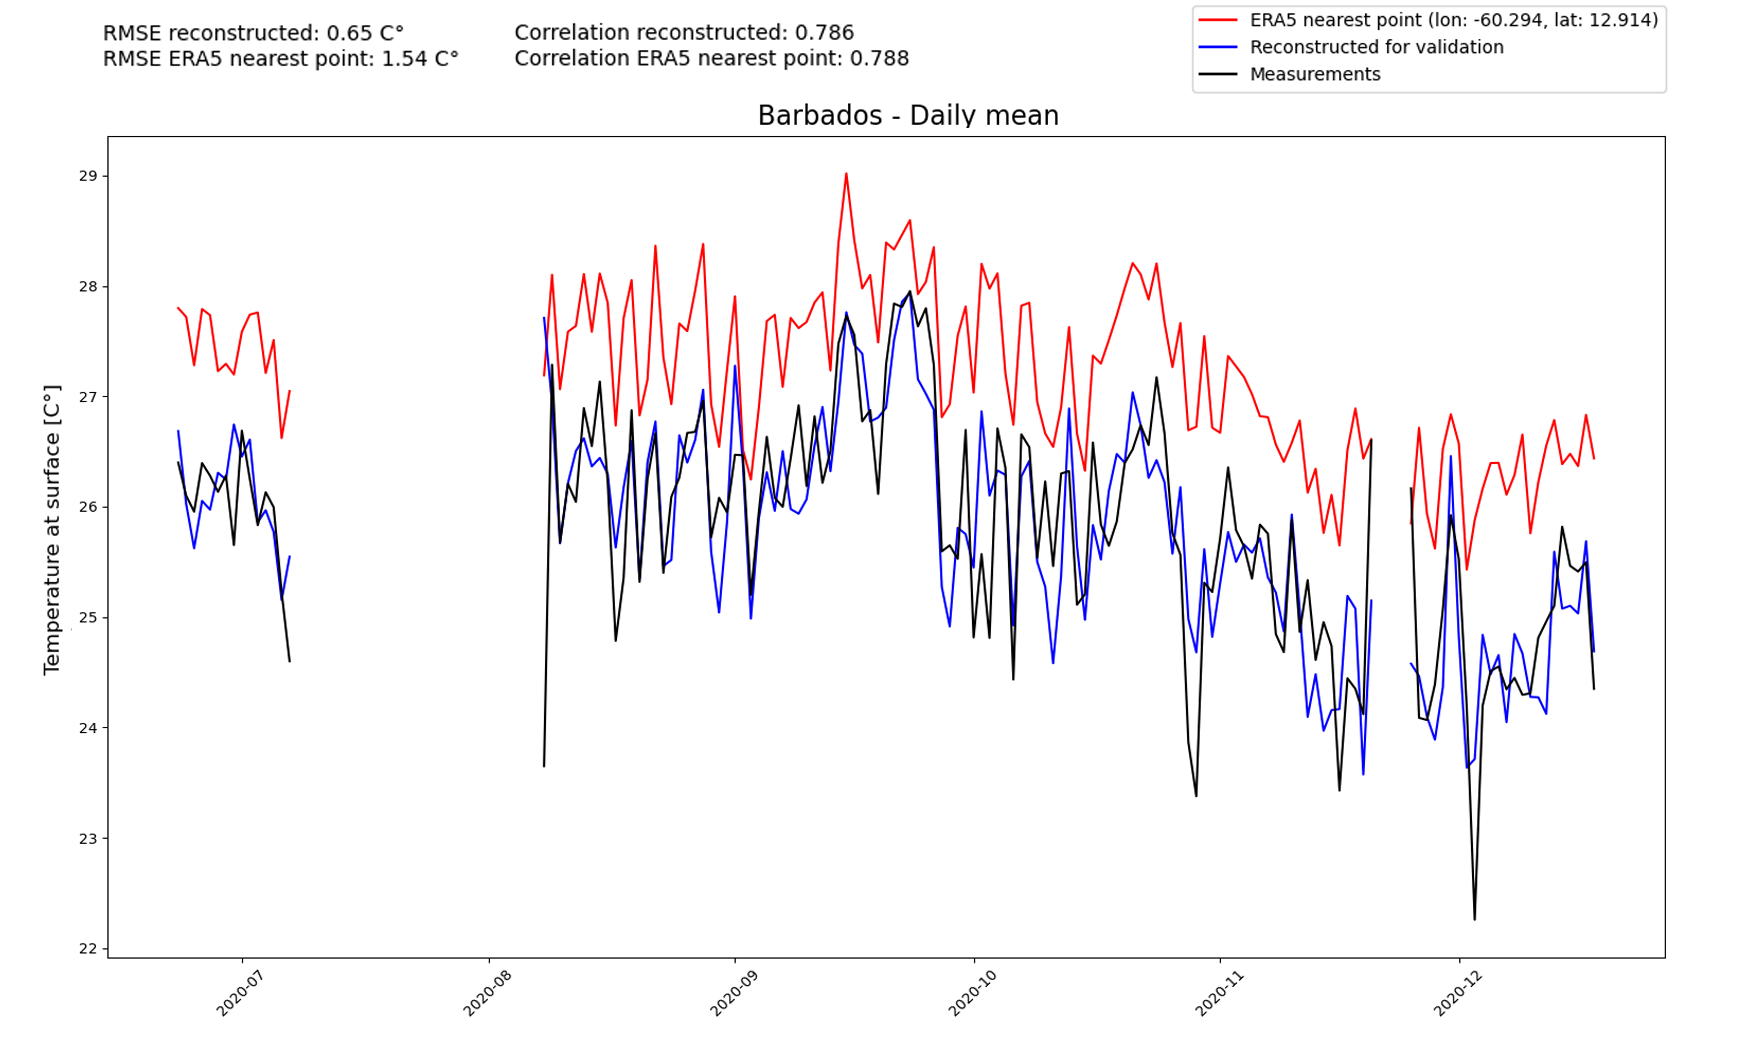
\includegraphics[width=\textwidth]{resources/images/charts/barbados_eval_grib_final/Barbados - Daily mean.png}
    \caption{Reconstructed temperature for Barbados-Station (Daily mean)}
\end{figure}

\begin{figure}
    \centering
    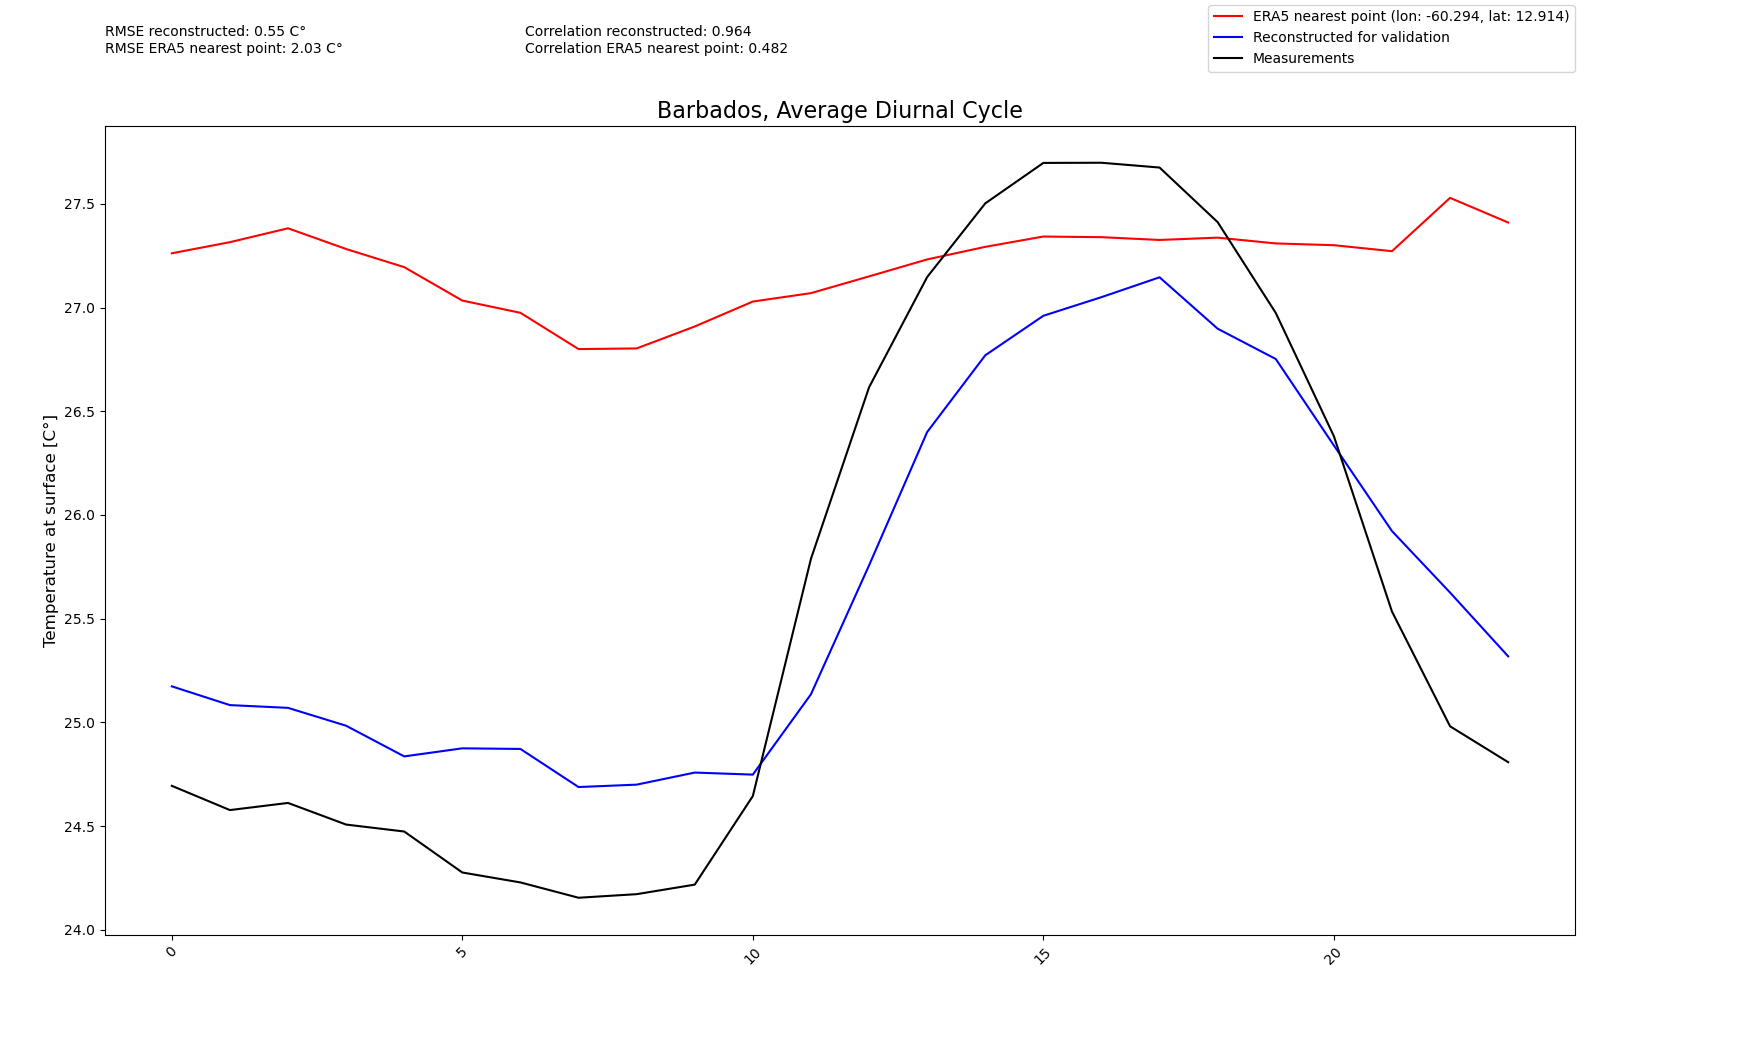
\includegraphics[width=\textwidth]{resources/images/charts/barbados_eval_grib_final/Barbados, Average Diurnal Cycle.png}
    \caption{Measured temperature for Barbados-Station (Average Diurnal Cycle)}
\end{figure}

\newpage

\subsection{Experimenting with time context}

\subsection{How to improve results}